%
% Neutron: quark ornac-pairs
%
%\begin{figure}
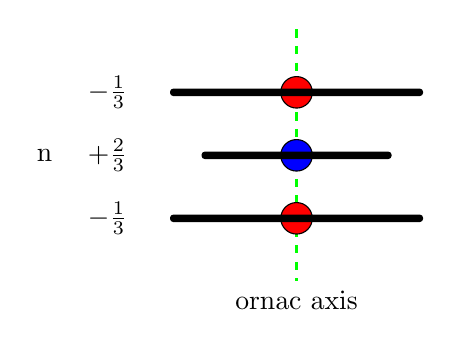
\begin{tikzpicture}[scale=0.4, rotate=0]



% Ornac axis
\draw[green, dashed, very thick] (4,4) -- (4,-4) ;
\path 
(4,-4) node [below]  {ornac axis};




\path 
(-4,0) node   {n};

% Down quark ornac-pair
\path 
(-2,2) node  (red) {$-\frac{1}{3}$};

\filldraw[fill=red, draw=black] (4,2) circle [radius=0.5];

\filldraw[fill=black, draw=black ,rounded corners=1pt] (0, 1.9) rectangle (8, 2.1);


% Up quark ornac-pair
\path 
(-2,0) node  (red) {$+\frac{2}{3}$};

\filldraw[fill=blue, draw=black] (4,0) circle [radius=0.5];

\filldraw[fill=black, draw=black ,rounded corners=1pt] (1,-0.1) rectangle (7, 0.1);



% Down quark ornac-pair
\path 
(-2,-2) node  (red) {$-\frac{1}{3}$};

\filldraw[fill=red, draw=black] (4,-2) circle [radius=0.5];

\filldraw[fill=black, draw=black ,rounded corners=1pt] (0, -1.9) rectangle (8, -2.1);




\end{tikzpicture}
\caption{Neutron from side build up off quark ornac-pairs 
\label{fig:Neutron  from side build up off quark ornac-pairs}}
%\end{figure}



